%!TEX root = ../thesis.tex


\section{Introduction}

\begin{figure}
    \centering
    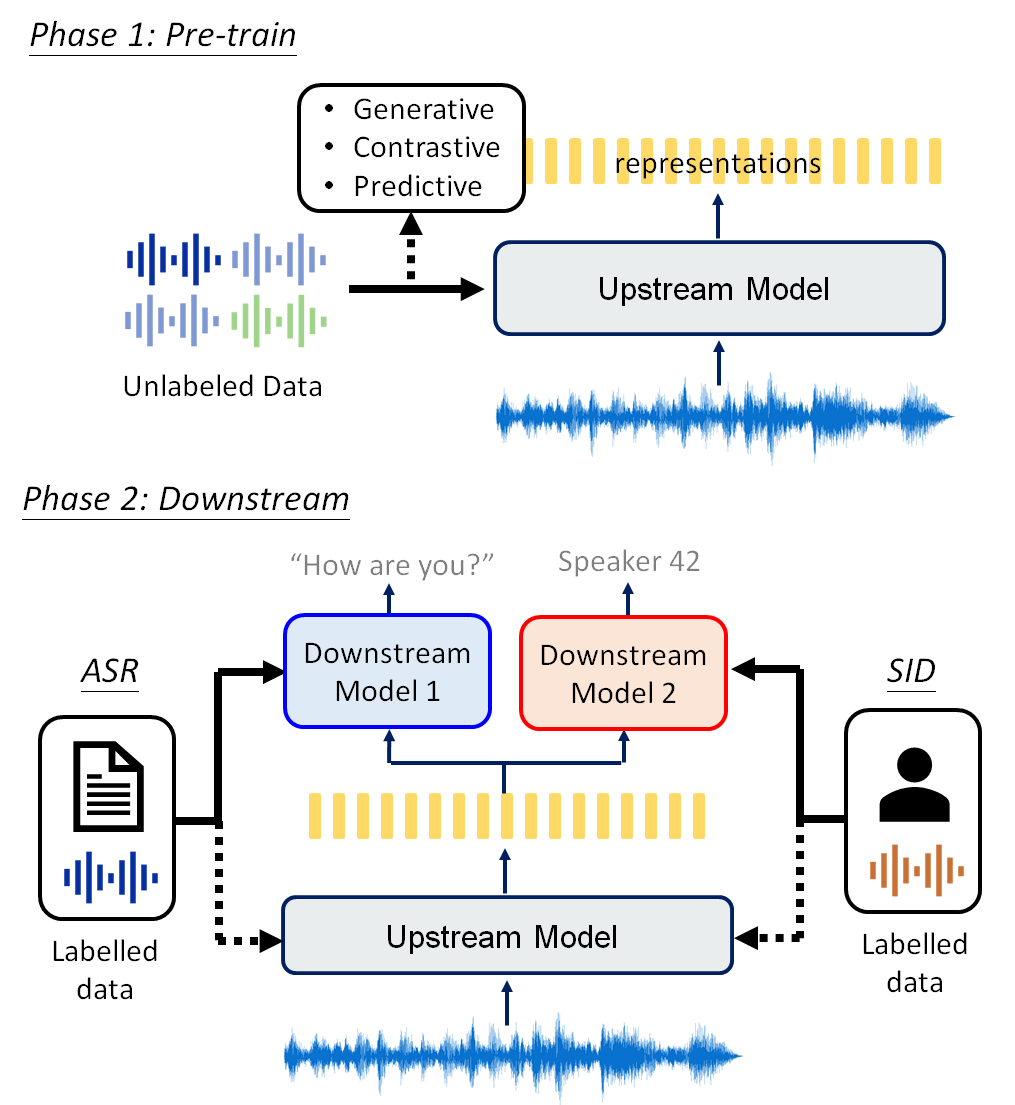
\includegraphics[width=0.80\textwidth]{paper_review/SSL_framework.png}
	 \caption{Framework for using self-supervised representation learning in
	 downstream applications}
    \label{fig:SSL_framework}
\end{figure}


Over the past decade, deep learning approaches have revolutionized speech processing
through a giant leap in performance, enabling various real-world applications.
Supervised learning of deep neural networks has been the cornerstone of this
transformation, offering impressive gains for scenarios rich in labeled
% data~\cite{lecun_deep_2015}. 
% data~\cite{lecun_deep_2015, hinton_deep_2012}. 
% data~\cite{bourlard_connectionist_1994}. 
% data~\cite{lecun_deep_2015,bourlard_connectionist_1994}. 
data~\cite{lecun_deep_2015,hinton_deep_2012,bourlard_connectionist_1994}. 
Paradoxically, this heavy reliance on supervised learning has restricted progress in
languages and domains that do not attract the same level of labeling
investment. 

To overcome the need for labeled data, researchers have explored approaches that use
unpaired audio-only data to open up new industrial speech use-cases and
low-resource languages~\cite{kemp_unsupervised_1999, lamel_lightly_2002, ma_unsupervised_2006}. Inspired by how
children learn their first language through listening and interacting with
family and surroundings, scientists seek to use raw waveforms and
spectral signals to learn speech representations that capture low-level
acoustic events, lexical knowledge, all the way to syntactic and semantic
information. These learned representations are then used for target downstream
applications requiring a minimal number of labeled data~\cite{hinton_learning_2007,
lecun_tutorial_2006, bengio_representation_2013}. 
Formally, representation learning refers to algorithms for extracting latent
features that capture the underlying explanatory factors for the observed
input~\cite{bengio_representation_2013}. 

Representation learning approaches are generally considered examples of \textit{unsupervised
learning}, which refers to the family of machine learning methods that discover
naturally occurring patterns in training samples for which there are no pre-assigned
labels or scores~\cite{jordan_machine_2015}. 
The term ``unsupervised'' is used to distinguish this family of methods from
``supervised'' approaches, which assign a label to each training sample, and
``semi-supervised'' approaches, which utilize a small number of training samples
with labels to guide learning using a larger volume of unlabeled samples.
Examples of unsupervised learning techniques include k-means clustering~\cite{gray_vector_1984}, mixture models~\cite{jordan_hierarchical_1994}, autoencoders~\cite{hinton_autoencoders_1994},
and non-negative matrix factorization~\cite{lee_learning_1999}. 
\textit{Self-supervised learning} (SSL) is a fast-growing subcategory of
unsupervised learning approaches, which are techniques that utilize
information extracted from the input data itself as the label to learn
representations useful for 
downstream tasks. {\color{black} For example, unsupervised k-means clustering doesn't adhere to this definition of self-supervision since it iteratively minimizes the within-cluster variance during learning.}
In this review, we
focus on self-supervised learning approaches.

\Cref{fig:SSL_framework} outlines self-supervised representation learning in
relation to downstream applications. 
There are two stages in this framework.
In the first stage, we use SSL to pre-train a \textit{representation model},
also called an \textit{upstream model} or a \textit{foundation model}.
In the second stage, downstream tasks use either the learned
representation from the frozen model, or fine-tune the entire pre-trained model
in a supervised phase~\cite{hinton_reducing_2006}. 
Automatic speech recognition (ASR) and speaker identification (SID) are 
examples of downstream applications in \cref{fig:SSL_framework}.

It is considered desirable for learned speech representations to be
disentangled, invariant, and hierarchical.
Since spoken utterances contain much richer information than the corresponding text
transcriptions---e.g., speaker identity, style, emotion, surrounding noise, and
communication channel noise---it is important to learn representations that
disentangle these factors of variation. Furthermore, invariance of the learned
features to changes in background noise and in the communication channel ensures
stability with respect to downstream application scenarios. Learning feature
hierarchies at the acoustic, lexical, and semantic levels supports applications
with different requirements. For instance, whereas a speaker identification task
benefits from a low-level acoustic representation, a speech
translation task requires a more semantic representation of the input
utterance. 

Due to the popularity of SSL, reviews have been published about the
technology in general~\cite{bommasani_opportunities_2021,ericsson_selfsupervised_2022,liu_selfsupervised_2021} as well as its application to natural language processing (NLP)~\cite{rogers_primer_2020,liu_pretrain_2021,xia_which_2020,qiu_pretrained_2020} and computer vision (CV)~\cite{jing_selfsupervised_2021}. Recently, a brief overview with a general focus on speech representation learning was published \cite{borgholt_brief_2022}. 
However, none of these overviews focus exclusively on SSL for speech processing. Since the speech signal differs greatly from image and text inputs, many  theories  and technologies have been developed to address the unique challenges of speech. 
One review addresses speech representation learning based on deep learning models~\cite{latif_deep_2021}, but does not address recent developments in self-supervised learning. This motivates this overview of speech SSL.


The structure of this paper is arranged as follows. \Cref{sec:thirdwave}
briefly reviews the history of speech representation learning, and
\cref{sec:approach} reviews current speech SSL models.
\Cref{section:benchmark} surveys SSL datasets and benchmarks, 
and discusses and compares results from different works. \Cref{analysis}
analyzes successful SSL approaches and offers insights into the
importance of technological innovations. \Cref{sec:zero} reviews 
zero-resource downstream tasks that utilize SSL. 
Finally, \cref{sec:conclusion} summarizes the paper and suggests 
future research directions.


